\chapter{ROS 2 Middleware}

    A significant change from \ac{ROS} 1 to \ac{ROS} 2 is the shift from a custom transport layer consisting of \ac{TCPROS} to \ac{DDS}. \ac{DDS} is a publish-subscribe communication standard defined by \ac{OMG}. \ac{DDS} uses \ac{IDL} for defining and serializing messages~\cite{rosondds}. In contrast to \ac{ROS} 1, which requires a \ac{ROS} master in order for nodes to discover and communicate with each other, \ac{ROS} 2 discovery system is handled by \ac{DDS} and each of the \ac{DDS} vendors provides different options for customizing the communication layer.

    One notable advantage of moving away from a custom transport protocol is that the \ac{ROS} client libraries are now agnostic to the middleware interface; this means that the complexities of the \ac{DDS} implementation are not exposed to the end user~\cite{ros2middle}. As a consequence, multiple middleware interfaces can be implemented as long as they fulfill the following requirements: 
    \begin{itemize}
        \item publishing and subscribing
        \item message serialization
        \item discovery
    \end{itemize}\label{ite:rmwreqs}
    
    The interaction between the \ac{ROS} user, the \ac{ROS} client libraries, and the middleware layers is shown in Figure~\ref{fig:middleware}.

    \begin{figure}[htbp]
        \centering
        \vspace{1em}
        \begin{tikzpicture}
            \node (user) [packBox] {ROS User};

            \node (rcl) [packBox, yshift=-2cm] {ROS Client Libraries \\ \small\textsf{rclcpp | rclpy}};

            \node (interface) [packBox, yshift=-4cm] {Middleware Interface \\ \small\textsf{rmw}};

            \node (implementation) [packBox, yshift=-6cm] {\textbf{Middleware Implementation} \\ \small\textsf{fastrtps | cyclonedds | connextdds | gurumdds | custom}};

            \begin{scope}[transform canvas={xshift=-0.5cm}]
                \draw [-to] (user) -- (rcl);
                \draw [-to] (rcl) -- (interface);
                \draw [-to] (interface) -- (implementation);
            \end{scope}

            \begin{scope}[transform canvas={xshift=0.5cm}]
                \draw [to-] (user) -- (rcl);
                \draw [to-] (rcl) -- (interface);
                \draw [to-] (interface) -- (implementation);
            \end{scope}

        \end{tikzpicture}
        \vspace{1em}
        \caption{Relations between the user, the \ac{ROS} client libraries and the middleware packages~\cite{ros2middle}.}
        \label{fig:middleware}
    \end{figure}


\section{Supported Implementations}

    Currently, \ac{ROS} 2 releases provide full support for three middleware implementations: eProsima Fast \ac{DDS}, Eclipse Cyclone \ac{DDS}, and \ac{RTI} Connext \ac{DDS}. The binaries also support Gurum \ac{DDS}, but the implementation requires a separate installation~\cite{docsdds}. 

    \subsection{eProsima Fast DDS}

    eProsima Fast \ac{DDS}, also known as Fast \ac{RTPS}, is the default middleware implementation for \ac{ROS} 2 packages. Some of the main advantages of Fast \ac{DDS} is that it is free, open source, and it is developed for most platforms including Linux, Windows, Mac OS, and QNX. A rich set of \ac{QoS} parameters is also available for tuning the communication protocols to any particular system. Fast \ac{DDS} follows a \ac{DCPS} model, which consists four elements: publishers, subscribers, topics, and domains~\cite{dcps}. This model introduces the concept of \textsf{Data Writers} and \textsf{Data Readers} which, as the names imply, have read and write permissions to the ``Global Data Space'' as specified by the \ac{DDS} standard~\cite{introdds}. Figure~\ref{fig:ddsdomain} displays an example of the Fast \ac{DDS} architecture and demonstrates how the different elements interact with each other.

    \begin{figure}[htbp]
        \centering
        \vspace{1em}
        \begin{tikzpicture}
            \node (domain) [
                box, 
                minimum width=14cm,
                text depth=6cm,
                fill=igmrLightBlue!10!bgColor,
            ] {DDS Domain};
            
            \node (p1) [
                box,
                xshift=-4cm,
                minimum width = 4cm,
                text depth=4.5cm,
                fill=igmrLightBlue!40!bgColor,
            ] {Domain Participant};

            \node (pub1) [
                box,
                xshift=-4cm,
                yshift=0.5cm,
                minimum width=3.5cm,
                text depth=1cm
            ] {Publisher};

            \node (dw1) [
                box,
                xshift=-4cm,
                yshift=0.2cm,
                minimum width=3cm,
                fill=bgColor,
            ] {Data Writer};

            \node (sub1) [
                box,
                xshift=-4cm,
                yshift=-1.5cm,
                minimum width=3.5cm,
                text depth=1cm
            ] {Subscriber};

            \node (dr1) [
                box,
                xshift=-4cm,
                yshift=-1.8cm,
                minimum width=3cm,
                fill=bgColor,
            ] {Data Reader};

            \node (p2) [
                box,
                xshift=4cm,
                minimum width=4cm,
                text depth=4.5cm,
                fill=igmrLightBlue!40!bgColor,
            ] {Domain Participant};

            \node (sub2) [
                box,
                xshift=4cm,
                yshift=0.5cm,
                minimum width=3.5cm,
                text depth=1cm
            ] {Subscriber};

            \node (dr2) [
                box,
                xshift=4cm,
                yshift=0.2cm,
                minimum width=3cm,
                fill=bgColor,
            ] {Data Reader};

            \node (t1) [
                box,
                minimum width=2cm,
                minimum height=1cm,
                fill=igmrLightBlue!40!bgColor,
            ] {Topic};

            \node (dot1) [
                rectangle,
                xshift=-1.5cm,
            ] {};

            \draw [thick] (t1) -- (dot1.center);
            \draw [arrow] (dw1.east) -- (dw1.east-|t1.west);
            \draw [arrow] (dot1.center) |- (dr1);
            \draw [arrow] (t1.east|-dr2.west) -- (dr2.west);

        \end{tikzpicture}
        \vspace{1em}
        \caption{Instance of a typical Fast \ac{DDS} domain model.}
        \label{fig:ddsdomain}
    \end{figure}

    \subsection{Eclipse Cyclone DDS}

        Similar to Fast \ac{DDS}, Cyclone \ac{DDS} is free and open source and supports the three major platforms, Linux, Windows, and Mac OS. Cyclone \ac{DDS} offers a ``data-centric'' architecture with space- and time-decoupling with a zero configuration discovery system~\cite{eclipse}. Additionally, this implementation includes Python bindings to simplify the definition of data types. 

    \subsection{RTI Connext DDS}

        Unlike the previously mentioned \ac{DDS} implementations, \ac{RTI} Connext DDS requires a separate installation plus the purchase of a license, however, free licenses are available for researchers and academics~\cite{connextuni}. \ac{RTI} also offers a variety of tools to \ac{ROS} users including admin consoles, system monitors, and recording and routing services~\cite{rtiblog}.

    \subsection{Gurum Networks Gurum DDS}

        The last implementation which is supported by the \ac{ROS} 2 binaries is GurumDDS. And as in the case of Connext DDS, GurumDDS also requires its own installation after the purchase of a license, although, free trials are available~\cite{gurum}. 


\section{Custom Middleware}

    Out of the aforementioned middleware implementations, none of them have targeted the web browser as the basis for the \ac{DDS} Global Data Space. There exists a \ac{WebDDS} standard, also specified by \ac{OMG}, which dictates how a \ac{DDS} system can be exposed to web clients via a \ac{WebDDS} service~\cite{webdds}. However, this setup would still require a native \ac{DDS} system. As an alternative to \ac{DDS}, custom middleware packages can be implemented as long as they meet the basic requirements listed in Section~\ref{ite:rmwreqs}.

    \subsection{Email}

        An excellent example of a middleware implementation which is not based on the \ac{DDS} standard is \textsf{rmw\_email}. With this implementation, all of the \ac{ROS} 2 communications for publishing and subscribing to topics and to call and respond to services are handled by sending emails. 

        \begin{figure}[htbp]
            \centering
            \begin{subfigure}[t]{0.49\textwidth}
                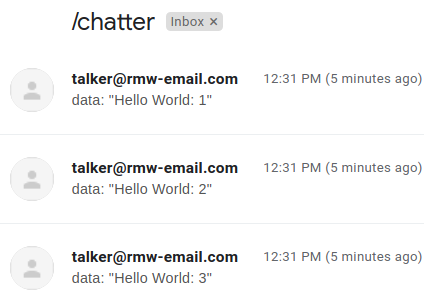
\includegraphics[height=0.68\textwidth]{05_email_pub.png}
                \caption{Email publisher}
            \end{subfigure}
            \begin{subfigure}[t]{0.49\textwidth}
                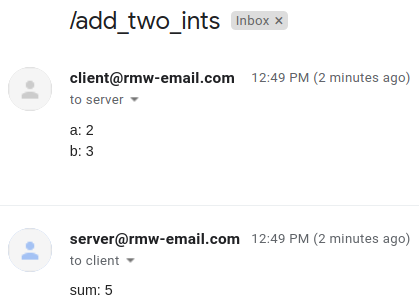
\includegraphics[height=0.68\textwidth]{05_email_srv.png}
                \caption{Email service client and server}
            \end{subfigure}
            \vspace{1em}
            \caption{Email \ac{RMW} implementation.}
            \label{fig:email}
        \end{figure}

        The implementation consists of two parts: \textsf{email} for handling the communications and \textsf{rmw\_email} which acts as an adapter to interface with \textsf{rmw}~\cite{emailblog}. Figure~\ref{fig:email} shows a \ac{ROS} publisher, a service client, and a service server using this \textsf{email} middleware. Although \textsf{rmw\_email} does not reach the level of performance of the standard \ac{DDS} implementations, it showcases the flexibility of the additional abstraction layer integrated in \ac{ROS} 2 to support various middleware designs.


    \subsection{Zenoh}

        Continuing the trend of non-\ac{DDS} middleware implementations, another approach involves the use of Eclipse Zenoh. Zenoh is a publication, subscription and query protocol to unify data which can be used in embedded micro-controllers or even data centers~\cite{zenoh}. Open Robotics has tested the potential of using Zenoh as a middleware for ROS 2 applications and concluded that it could alleviate some of the common problems encountered with the default \ac{DDS} implementations by providing the users with hassle-free experience which does not require configuration and tuning unlike its \ac{DDS} counterparts~\cite{ros2zenoh}.

        Similar to \textsf{rmw\_email}, the interface between Zenoh and \ac{ROS} 2 is handled by \textsf{rmw\_zenoh}. As of 2023, \textsf{rmw\_zenoh} still remains in the experimental phase. One notable aspect of this implementation, is the adaptation of Fast CDR to provide type support for Zenoh.

    \subsection{Minimal Middleware Implementation}\label{ssec:minimal}

        The development of a custom middleware implementations consist of two major parts: the creation of a middleware ``adapter'' to communicate with the \ac{ROS} 2 middleware interface, and the formation of the middleware implementation itself. An overview of a custom middleware architecture is demonstrated in Figure~\ref{fig:rmwarch}. 

        \begin{figure}[htbp]
            \centering
            \vspace{1em}
            \begin{tikzpicture}
                \node (rmw) [packBox] {ROS 2 Middleware Abstraction Interface \\ \small\textsf{rmw}};

                \node (custom) [
                    rectangle,
                    rounded corners,
                    yshift=-3.5cm,
                    minimum width=12cm,
                    text width=11.5cm,
                    text height=4.5cm,
                    draw=textColor,
                    align=justify,
                    fill=igmrLightBlue!10!bgColor,
                ] {Custom Middleware};

                \node (rmwwasm) [
                    packBox, 
                    yshift=-2.3cm,
                    fill=igmrLightBlue!40!bgColor,
                ] {Middleware Adapter \\ \small\textsf{rmw\_email | rmw\_zenoh | rms\_wasm}};

                \node (interface) [
                    packBox, 
                    yshift=-4.3cm,
                    fill=igmrLightBlue!40!bgColor,
                ] {Middleware Implementation \\ \small\textsf{Email | Zenoh | Web Browser}};

                \begin{scope}[transform canvas={xshift=-0.5cm}]
                    \draw [arrow] (rmw) -- (rmwwasm);
                    \draw [arrow] (rmwwasm) -- (interface);
                \end{scope}

                \begin{scope}[transform canvas={xshift=0.5cm}]
                    \draw [arrow] (rmwwasm) -- (rmw);
                    \draw [arrow] (interface) -- (rmwwasm);
                \end{scope}

            \end{tikzpicture}
            \vspace{1em}
            \caption{Architecture overview of a \ac{ROS} 2 custom middleware implementation.}
            \label{fig:rmwarch}
        \end{figure}

        There are no standardized guidelines for how the middleware implementation should be formatted or what platforms it should support. The design of the implementation is highly dependent on the use case of the \ac{ROS} application. The only design requirements are that the implementation should have the means to publish and subscribe data, perform message serialization from and to \ac{ROS} message types, and have a discovery system to detect other participants in the specified domain. For this project, all of the communications are handled by the web browser and thus, the middleware is implemented in JavaScript.

        For the creation of a middleware ``adapter,'' \textsf{rmw} provides a set of primitives which are needed for higher level \ac{ROS} \ac{API}s. Generating the adapter requires implementing all of the relevant interface functions defined by \textsf{rmw}. Figures~\ref{fig:funinit} through~\ref{fig:funclient} highlight a few of the necessary interface functions. 

        % \lstset{
        %     columns=fullflexible,
        %     numbers=none,
        %     backgroundcolor=\color{lightgray!15!bgColor},
        %     xleftmargin=10pt,
        %     xrightmargin=10pt,
        %     frame=lrtb,
        %     framesep=10pt,
        %     framerule=0pt,
        %     % emph={int,char,double,float,unsigned,void,bool,const,uint,string},
        %     % emphstyle=\color{blue},
        %     emph={
        %         rmw_context_t, 
        %         rmw_ret_t, 
        %         rmw_init_options_t,
        %         rmw_node_t,
        %         rmw_guard_condition_t,
        %         size_t,
        %         rmw_publisher_t,
        %         rmw_publisher_allocation_t,
        %         rmw_publisher_options_t,
        %         rmw_qos_profile_t,
        %         rosidl_message_type_support_t,
        %         rmw_subscription_t,
        %         rmw_subscription_allocation_t,
        %         rmw_subscription_options_t,
        %         },
        %     emphstyle=\color{gray!60!textColor},
        % }


        \begin{figure}[htbp]
            \begin{lstlisting}[language=C++]
// Return a zero initialized context structure
rmw_context_t 	rmw_get_zero_initialized_context (void) {...}

// Initialize the middleware with the given options and yield a context
rmw_ret_t 	rmw_init (
    const rmw_init_options_t *options, 
    rmw_context_t *context) {...}
    
// Shutdown the middleware for a given context
rmw_ret_t 	rmw_shutdown (rmw_context_t *context) {...}

// Finalize a context
rmw_ret_t 	rmw_context_fini (rmw_context_t *context) {...}

// Return a zero initialized init options structure
rmw_init_options_t 	rmw_get_zero_initialized_init_options (void) {...}

// Initialize given init_options with the default values and implementation specific values
rmw_ret_t 	rmw_init_options_init (
    rmw_init_options_t *init_options, 
    rcutils_allocator_t allocator) {...}

// Copy the given source init options to the destination init options
rmw_ret_t 	rmw_init_options_copy (
    const rmw_init_options_t *src, 
    rmw_init_options_t *dst) {...}

// Finalize the given init_options
rmw_ret_t 	rmw_init_options_fini (rmw_init_options_t *init_options) {...}\end{lstlisting}
            \caption{Functions for initialization and shutdown.}
            \label{fig:funinit}
        \end{figure}


        \begin{figure}[htbp]
            \begin{lstlisting}[language=C++]
// Create a node and return a handle to that node
rmw_node_t * 	rmw_create_node (
    rmw_context_t *context, 
    const char *name, 
    const char *namespace_, 
    size_t domain_id, 
    bool localhost_only) {...}

// Finalize a given node handle, reclaim the resources, and deallocate the node handle
rmw_ret_t 	rmw_destroy_node (rmw_node_t *node) {...}

// Return a guard condition which is triggered when the ROS graph changes
const rmw_guard_condition_t * 	rmw_node_get_graph_guard_condition (
    const rmw_node_t *node) {...}
\end{lstlisting}
            \label{fig:funnode}
            \caption{Node functions.}
        \end{figure}


        \begin{figure}[htbp]
            \begin{lstlisting}[language=C++]
// Create and return an rmw publisher
rmw_publisher_t * 	rmw_create_publisher (
    const rmw_node_t *node, 
    const rosidl_message_type_support_t *type_support, 
    const char *topic_name, 
    const rmw_qos_profile_t *qos_policies, 
    const rmw_publisher_options_t *publisher_options) {...}

// Destroy publisher
rmw_ret_t 	rmw_destroy_publisher (
    rmw_node_t *node, 
    rmw_publisher_t *publisher) {...}

// Initialize a publisher allocation to be used with later publications
rmw_ret_t 	rmw_init_publisher_allocation (
    const rosidl_message_type_support_t *type_support, 
    const rosidl_runtime_c__Sequence__bound *message_bounds, rmw_publisher_allocation_t *allocation) {...}

// Destroy a publisher allocation object
rmw_ret_t 	rmw_fini_publisher_allocation (
    rmw_publisher_allocation_t *allocation) {...}

// Return a rmw_publisher_options_t initialized with default values
rmw_publisher_options_t 	rmw_get_default_publisher_options (void) {...}

// 	Publish a given ros_message
rmw_ret_t 	rmw_publish (
    const rmw_publisher_t *publisher, 
    const void *ros_message, 
    rmw_publisher_allocation_t *allocation) {...}
\end{lstlisting}
            \caption{Publisher functions.}
            \label{fig:funpub}
        \end{figure}


        \begin{figure}[htbp]
            \begin{lstlisting}[language=C++]
// Create and return an rmw subscription
rmw_subscription_t * 	rmw_create_subscription (
    const rmw_node_t *node, 
    const rosidl_message_type_support_t *type_support, 
    const char *topic_name, 
    const rmw_qos_profile_t *qos_policies, 
    const rmw_subscription_options_t *subscription_options) {...}

// Destroy subscription
rmw_ret_t 	rmw_destroy_subscription (
    rmw_node_t *node, 
    rmw_subscription_t *subscription) {...}

// Retrieve the number of matched publishers to a subscription
rmw_ret_t 	rmw_subscription_count_matched_publishers (
    const rmw_subscription_t *subscription, 
    size_t *publisher_count) {...}

// Retrieve the actual qos settings of the subscription
rmw_ret_t 	rmw_subscription_get_actual_qos (
    const rmw_subscription_t *subscription, 
    rmw_qos_profile_t *qos) {...}

// Take an incoming message from a subscription
rmw_ret_t 	rmw_take (
    const rmw_subscription_t *subscription, 
    void *ros_message, 
    bool *taken, 
    rmw_subscription_allocation_t *allocation) {...}
\end{lstlisting}
            \caption{Subscriber functions.}
            \label{fig:funsub}
        \end{figure}

        \begin{figure}[htbp]
            \begin{lstlisting}[language=C++]
// Create an rmw service server that responds to requests
rmw_service_t * 	rmw_create_service (
    const rmw_node_t *node, 
    const rosidl_service_type_support_t *type_support, 
    const char *service_name, 
    const rmw_qos_profile_t *qos_policies) {...}

// 	Destroy and unregister the service from this node
rmw_ret_t 	rmw_destroy_service (
    rmw_node_t *node, 
    rmw_service_t *service) {...}

// Attempt to take a request from this service's request buffer
rmw_ret_t 	rmw_take_request (
    const rmw_service_t *service, 
    rmw_service_info_t *request_header, 
    void *ros_request, 
    bool *taken) {...}

// 	Send response to a client's request
rmw_ret_t 	rmw_send_response (
    const rmw_service_t *service, 
    rmw_request_id_t *request_header, 
    void *ros_response) {...}
\end{lstlisting}
            \caption{Service server functions.}
            \label{fig:funsrv}
        \end{figure}


        \begin{figure}[htbp]
            \begin{lstlisting}[language=C++]
// Create an rmw client to communicate with the specified service
rmw_client_t * 	rmw_create_client (
    const rmw_node_t *node, 
    const rosidl_service_type_support_t *type_support, 
    const char *service_name, 
    const rmw_qos_profile_t *qos_policies) {...}

// Destroy and unregister a service client
rmw_ret_t 	rmw_destroy_client (
    rmw_node_t *node, 
    rmw_client_t *client) {...}

// Send a service request to the rmw server
rmw_ret_t 	rmw_send_request (
    const rmw_client_t *client, 
    const void *ros_request, 
    int64_t *sequence_id) {...}

// Attempt to get the response from a service request
rmw_ret_t 	rmw_take_response (
    const rmw_client_t *client, 
    rmw_service_info_t *request_header, 
    void *ros_response, 
    bool *taken) {...}

// Check if a service server is available for the given service client
rmw_ret_t 	rmw_service_server_is_available (
    const rmw_node_t *node, 
    const rmw_client_t *client, 
    bool *is_available) {...}
\end{lstlisting}
            \caption{Service client functions.}
            \label{fig:funclient}
        \end{figure}


    \pagebreak
    Besides the essential functions for creating and destroying nodes, publishers, subscribers, and services, there exists additional functions to handle events, wait sets, guard conditions, \ac{QoS} policies, and allocators. Additionally, there are utility functions and macros for handling errors, customizing log outputs and name validation. A full list of functions can be found in the \textsf{rmw} \ac{API} documentation~\cite{rmwapi} TODO: or appendix??.

\pagebreak
\section{Substituting ROS 2 Middleware}

    There are two methods of using a particular middleware implementations when launching \ac{ROS} applications other than the default implementation. The first method requires setting the environment variable \small\textsf{RMW\_IMPLEMENTATION} to the implementation identifier of choice. An example of how to launch a publisher node with this method is shown in Figure~\ref{fig:envrmw}.

    \begin{figure}[thbp]
        \centering
            \begin{lstlisting}[
                language=bash,
                frame=lrtb,
                framesep=10pt,
                framerule=0pt,
                emph={RMW_IMPLEMENTATION},
                emphstyle=\color{blue},
            ]
RMW_IMPLEMENTATION=rmw_connextdds ros2 run demo_nodes_cpp talker
\end{lstlisting}
        \caption{Launching a node with Connext \ac{DDS}.}
        \label{fig:envrmw}
    \end{figure}

    Nonetheless, the caveat of this first method is that the \ac{ROS} 2 binaries installed must have support for the specified implementation~\cite{subrmw}. Alternatively, the second method involves rebuilding all of the desired \ac{ROS} 2 packages from source and specify the \small\textsf{RMW\_IMPLEMENTATION} as a CMake argument. When building from source, if the packages for multiple \ac{RMW} implementations are available, all of them will be built starting with Fast \ac{DDS} as the default. If Fast \ac{DDS} is not available, then the default implementation will be selected by the next available implementation identifier in alphabetical order~\cite{docsdds}. To ensure that only a single implementation is available for use, the simplest solution is to explicitly ignore or remove the packages belonging to undesired implementations from the workspace.
